\documentclass{beamer}
\usepackage[utf8]{inputenc}
\usepackage{epsfig}
\usepackage{graphicx}
\usepackage{amsmath,amsthm,amsfonts,amssymb,amscd}
\usepackage{lastpage}
\usepackage{enumerate}
\usepackage{fancyhdr}
\usepackage{mathrsfs}
\usepackage{xcolor}
\usepackage[ruled,vlined]{algorithm2e}
\usepackage{graphicx}
\usepackage{listings}
\usepackage{float}
\usepackage{hyperref}
\usepackage{appendixnumberbeamer}
\usepackage[section]{placeins}

\DeclareMathOperator{\tr}{tr}
\DeclareMathOperator*{\argmin}{arg\,min}
\DeclareMathOperator*{\argmax}{arg\,max}
\newtheorem{thm}{Theorem}
\newtheorem{dfn}{Definition}
\newtheorem{lem}{Lemma}
\usetheme{boadilla}
\usecolortheme{whale}

%Information to be included in the title page:
\title[DMD and Network Evolution]{Dynamic Mode Decomposition and Network Evolution}
\author{Robert Simpson}
\institute{San Diego State University}
\date{Spring 2021}

%\logo{\includegraphics[height=1.5cm]{SDSUprimary3Crgb.png}}

\begin{document}
\frame{\titlepage}

\begin{frame}
\tableofcontents
\end{frame}

\section{Purpose}
\begin{frame}
    \frametitle{Purpose}
    Purpose: We want to characterize local network dynamics via motif interactions and extract
    the spatiotemporal coherent structures using
    the Dynamic Mode Decomposition (DMD) and Kernel Dynamic Mode Decomposition (KDMD) algorithms.
    We analyze the results using the reconstruction error and the individual mode error.
    \end{frame}
\section{Motifs}


%%Review
\begin{frame}
    \frametitle{Graph Theory}
    \begin{definition}[Graph]
        Let $G = (V,E)$ be a graph with $V$ being a set of vertices (or nodes), 
        and $E$, a set of edges. If $v$ is a vertex of $G$ we write $v \in V(G)$. 
        If $u,v \in V(G)$ and there is an edge between $u$ and $v$ we 
        write $\{u,v\} \in E(G)$
    \end{definition}
    

    \begin{definition}[Adjacency Matrix]
        The adjacency matrix $A$ for any graph $G$ with $n=|V|$ vertices is a matrix of size
        $n \times n$. The element $a_{i,j}$ is defined to be
        $$
        a_{i,j} = 
        \begin{cases}
            1 \quad e_{i,j} \in E(G)\\
            0 \quad e_{i,j} \not \in E(G)\\
        \end{cases}
        $$
        \label{def:adjmat}
    \end{definition}
\end{frame}


\begin{frame}
\frametitle{Graph Homomorphisms and Isomorphisms}

 \begin{definition}[Homomorphism]
            We call $f: G \rightarrow H$ a homomorphism,
            if $f$ maps endpoints in $G=(V(G),E(G))$ to endpoints in $H=(V(H),E(H))$.
            i.e. $ \forall u,v \in V(G) \quad \{u,v\} \in E(G) \Rightarrow \{f(u),
            f(v)\} \in E(H)$.
 \end{definition}

\begin{definition}[Isomorphism]
    An isomorphism is a homomorphism that is also bijective.
\end{definition}

\end{frame}

\begin{frame}
    \frametitle{Subgraphs and Motifs}
     
    \begin{dfn}[Subgraph]
        Let $G=(V,E)$ be a graph. We call $G'=(V',E')$ a subgraph, denoted $G' \subset G$, if
        $V' \subseteq V \land E' \subseteq E \cap (V' \times V')$. Furthermore we call $G'$
        an induced subgraph of $G$ if $\forall u,v \in V'$, $\{u,v\}\in E \iff \{u,v\}\in E'$.
    \end{dfn}

     \begin{definition}[Motif]
         Let $G'' \subset G$ be an induced subgraph. If $G''$ is isomorphic to $G'$
         we call $G''$ and appearance of $G'$. Provided that the number of appearances, or count,
         of $G'$ is greater than some $N\in \mathbb{N}$ we call $G'$ a motif, or pattern.
     \end{definition}

     The number of appearances of motif $G'$ we call the $G'$ motif count.
\end{frame}

\begin{frame}
    \frametitle{Walks, Cycles, and Stars}
    \begin{definition}[Walk]
        A walk $W = \{v_0, e_1, v_1, \dots v_n\}$ is a sequence of edges and vertices of $G$ such that
        for $0 \leq k \leq n-1$ the edge $e_i = \{v_k, v_k+1\}$.
    \end{definition}

    \begin{definition}[Cycle]
        A cycle $C_n$ is a walk of $n$ vertices, whose first and last vertex are the same.
    \end{definition}
\end{frame}

\begin{frame}
    \frametitle{Walks, Cycles, and Stars Cont.}
    \begin{definition}[Bipartite Graph]
        A bipartite graph $K$ is defined to be such that the vertices of $K$ can be separated into
        two disjoint sets $U$ and $V$, where there is an edge from every node in $U$ to every node in $V$.
    \end{definition}

    \begin{definition}[Star Graph]
        A star $S_k$ is a bipartite graph such that one disjoint set $U$ contains one vertex, and the 
        the other set $V$ contains the remaining $k$ vertices.
    \end{definition}
\end{frame}
        
\begin{frame}
    \frametitle{Non-Simple Cycles}
     The non-simple cycle motifs and how to count them through the adjacency matrix is found in Alon et al \cite{alon}. 
    \begin{figure}
        \includegraphics[width = 0.5\linewidth]{../Images/mega_motif.png}
    \end{figure}
\end{frame}

\section{The Barabási–Albert Model}
\begin{frame}
    \frametitle{Complex Networks}
    \begin{itemize}
    \item Networks represent objects or people and connections between them.
    \item We can describe networks through graph theory.
    \item Complex networks are structurally (topologically) non-trivial. They are often scale-free,
        meaning their degree distributions follow a power-law.
    \end{itemize}
        
        The fraction $P$ of nodes in the network having $k$ connections is described by 

        $$
        P(k)= k^{-\gamma},\quad \gamma>0
        $$

\end{frame}

\begin{frame} %%% Preferential attachment mechanism
\frametitle{The Barabási–Albert Model}
The Barabási–Albert model implements a preferential attachment mechanism to generate a 
scale-free network. Most real-world models are shown to be scale-free \cite{barabasi2016network}.

\vspace{3mm}

The network is formed dynamically.
$m$ nodes are initialized at $t=0$ and at each subsequent time-step a new node is added to the network 
and attached to $k$ nodes.

\vspace{3mm}

The probability $p$ we attach to a node $n$ is determined by 
$$
p(n) = \frac{d_i}{\sum^{N}_{k=1}d_k}
$$
\end{frame}

\begin{frame}
    \frametitle{Motif counts of BA model with $k=1$}
    \begin{figure}
        \includegraphics[width=\linewidth]{../Images/pref_attach_1_counts.png}
    \centering
    \end{figure}
\end{frame}

% \begin{frame}
%     \frametitle{$k=1$ Results}
%     \begin{figure}
%         \includegraphics[width=0.6\linewidth]{../Images/graph_stats_pref_attach_8_1_300.png}
%     \centering
%     \end{figure}
% \end{frame}

% \begin{frame}
%     \frametitle{$k=1$ Results}
%     \begin{figure}
%         \includegraphics[width=0.7\linewidth]{../Images/final_pref1_centrality.png}
%     \centering
%     \end{figure}
% \end{frame}

\begin{frame}
    \frametitle{Motif counts of BA model with $k=2$}
    \begin{figure}
        \includegraphics[width=\linewidth]{../Images/pref_attach_2_counts.png}
    \centering
    \end{figure}
\end{frame}

% \begin{frame}
%     \frametitle{$k=1$ Results}
%     \begin{figure}
%         \includegraphics[width=0.6\linewidth]{../Images/graph_stats_pref_attach_10_2_300.png}
%     \centering
%     \end{figure}
% \end{frame}

% \begin{frame}
%     \frametitle{$k=1$ Results}
%     \begin{figure}
%         \includegraphics[width=0.7\linewidth]{../Images/final_pref2_centrality.png}
%     \centering
%     \end{figure}
% \end{frame}


\section{The Thij Model}

\begin{frame}
\frametitle{Twitter}
    \begin{itemize}
        \item Twitter is a social media platform. Users can follow other Twitter users. A user populates the feed of all 
        their followers with their tweets and retweets. 
        \item We wish to construct a network that shows original messages and their retweets, and model the temporal development
        of this network.
        \item New users need to be able to enter the network and either post message or retweet existing messages. Users already 
        in the network also have the capacity to retweet other users.  
    \end{itemize}
\end{frame}

%%11 minutes

\begin{frame}
\frametitle{The Thij Model}
    The Thij model implements a preferential attachment mechanism, as well as a
    superstar mechanism \cite{thij}. The latter was first proposed by Bhamidi \cite{Bhamidi_2015}. 
    \vspace{3mm}
    The Thij model seeks to simulation a retweet network within a community. The model begins
    with a single message node $u_0$. There are three possible events at every time step.
\end{frame}

\begin{frame}
    \frametitle{Thij Model Events}
    \begin{enumerate}
        \item T1: A user $u_i$ posts an original message node.
        \item T2: A new user $v_i$ retweets either an original message mode or a retweet of a message node.
        \item T3: An existing user $v_i$ retweets either an original message mode or a retweet of a message node.
    \end{enumerate}
\end{frame}

\begin{frame}
    \frametitle{Thij Event Probabilities}
    We assign probabilities to each event in the following way. Let $P(T_i)$
    denote probability of event $T_i$. Let $\lambda \geq 0$, $1\geq p \geq 0$.
    \begin{align*}
        P(T1) = \frac{\lambda}{1 + \lambda}\\
        P(T2) = \frac{p}{1 + \lambda}\\
        P(T3) = \frac{1-p}{1 + \lambda}\\
    \end{align*}
\end{frame}

\begin{frame}
    \frametitle{Thij Preferential Attachment and The Superstar Mechanism}
    \begin{itemize}
        \item The Thij model incoporates a superstar mechanism. The superstar mechanism 
            assigns probability $q$ to attach to a single message node $u_i$ and $1-q$ to all other nodes.
        \item Which message node is assigned probability $q$ is determined by ratio of its descendants
         to all retweets in the network. The more retweets a message node has, the more likely 
         its assigned the the superstar mechanism, and the more likely the message is to be retweeted. 
    \end{itemize}
\end{frame}

\begin{frame}
    \frametitle{Motif counts of Thij model with $\lambda=0.2$, $p=0.2$}
    \begin{figure}
        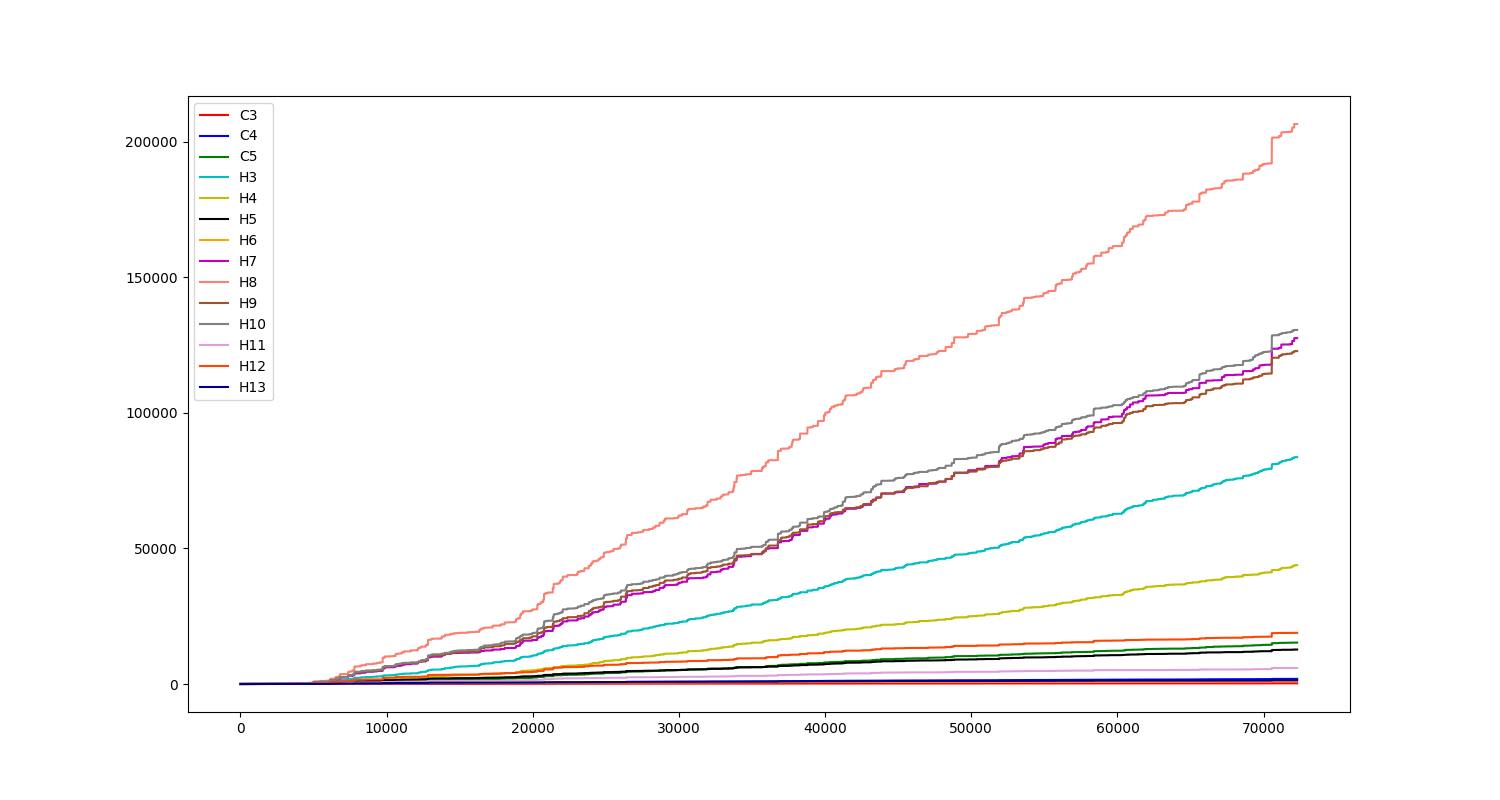
\includegraphics[width=\linewidth]{../Images/twitter_counts_020209.png}
    \centering
    \end{figure}
\end{frame}

\begin{frame}
    \frametitle{Motif counts of Thij model with $\lambda=0.2$, $p=0.8$}
    \begin{figure}
        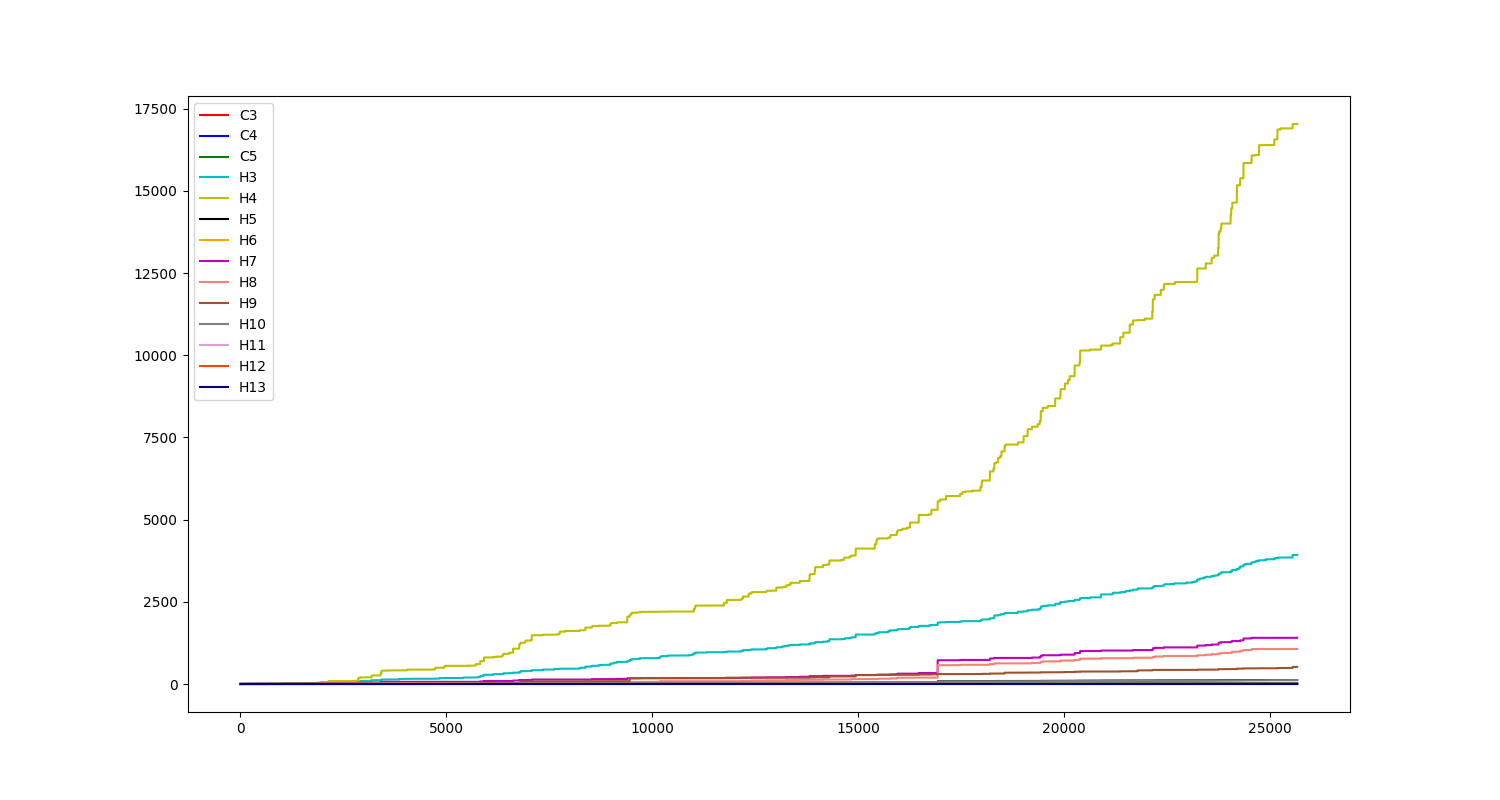
\includegraphics[width=\linewidth]{../Images/twitter_counts_020809.png}
    \centering
    \end{figure}
\end{frame}

\begin{frame}
    \frametitle{Motif counts of Thij model with $\lambda=0.8$, $p=0.2$}
    \begin{figure}
        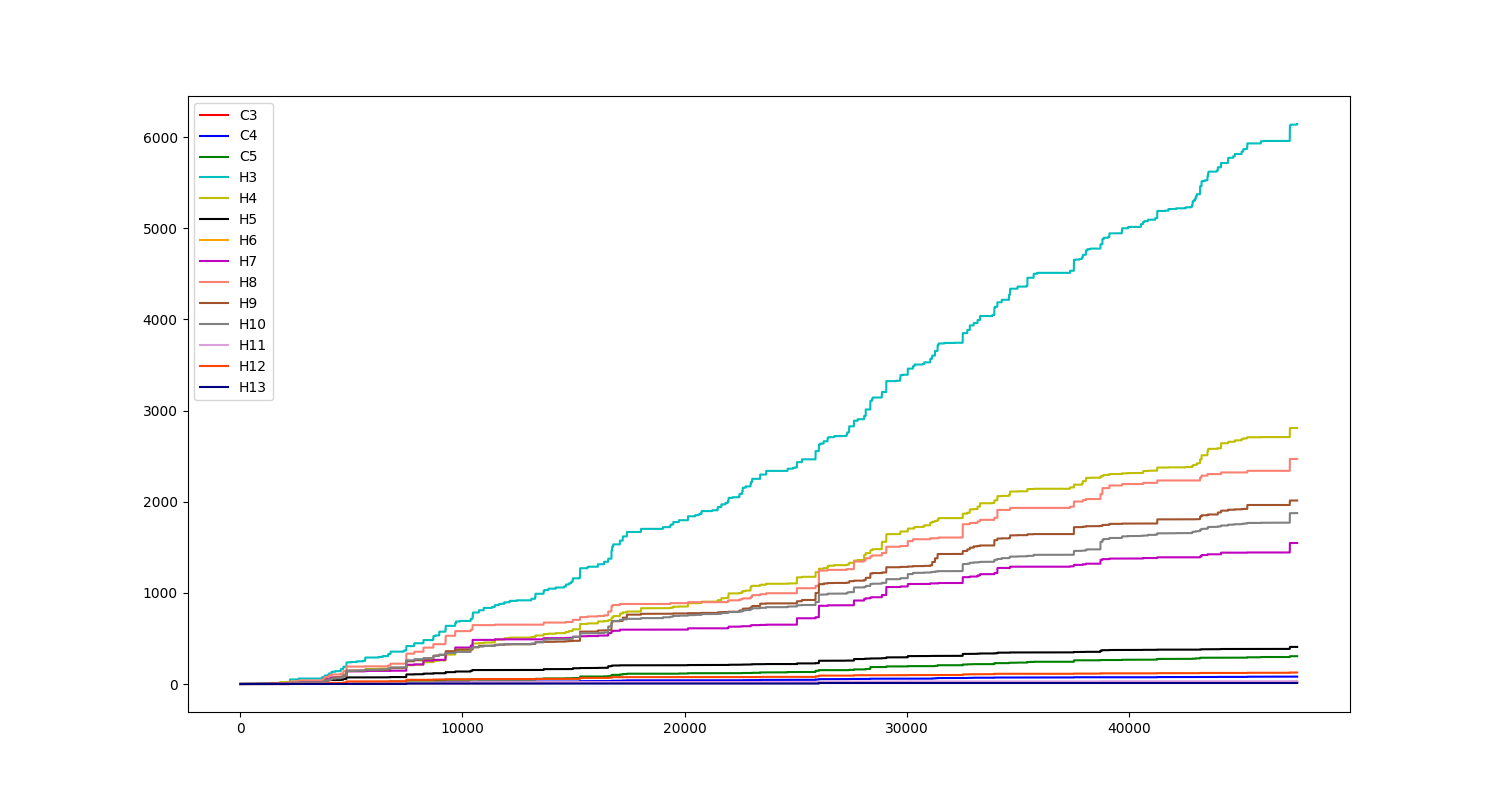
\includegraphics[width=\linewidth]{../Images/twitter_counts_080209.png}
    \centering
    \end{figure}
\end{frame}

\begin{frame}
    \frametitle{Motif counts of Thij model with $\lambda=0.8$, $p=0.8$}
    \begin{figure}
        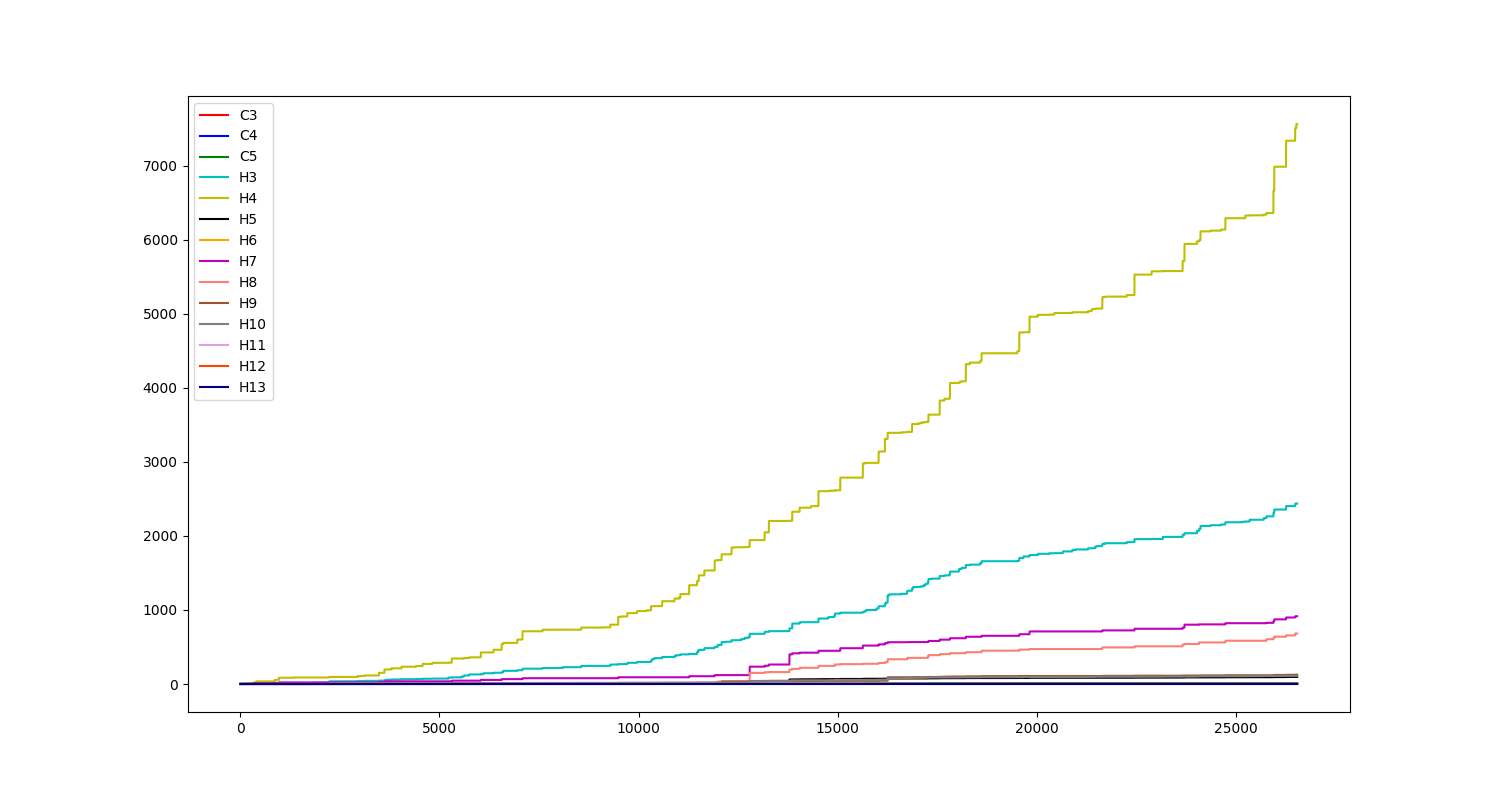
\includegraphics[width=\linewidth]{../Images/twitter_counts_080809.png}
    \centering
    \end{figure}
\end{frame}


% \section{The Effect of Node and Edge Addition}
% \begin{frame}
%     \frametitle{$T2$ events}
%     \begin{itemize}
%         \item The attachment of a node to a graph changes the number of appearances of motifs in the resulting graph.
%         \item The $$
%     \end{itemize}
        
% \end{frame}

% \begin{frame}
%     \frametitle{$H_4$ events}
    
% \end{frame}

% \begin{frame}
%     \frametitle{$H_7$ events}
    
% \end{frame}

% \begin{frame}
%     \frametitle{$H_8$ events}
    
% \end{frame}

\section{Covariance Between Motif Counts}
\begin{frame}
    \frametitle{The Covariance Matrix}
    
    \begin{definition}
        The element $C_{i,j}$ of the $i$th row and $j$th column of the covariance matrix $C \in \mathbb{R}^{n \times n}$
        is defined to be the covariance between $x_{i}$ and $x_j$, that is:
        $$
            C_{i,j} = \mathbf{E} ((x_i - \mathbf{E}(x_i))(x_j - \mathbf{E}(x_j)))
        $$
        $\mathbf{E}(x_i)$ denotes the expected value of the variable $x_i$. The value $C_{i,i}$ is called the variance of variable $x_i$.
        \label{def:cov}
    \end{definition}
\end{frame}
    

\begin{frame}
\frametitle{BA Model $k=1$}
\begin{figure}
    \includegraphics[width=0.6\linewidth]{../Images/CovMatPref1.png}
    \centering
\end{figure}
\end{frame}


\begin{frame}
    \frametitle{BA Model $k=2$}
    \begin{figure}
        \includegraphics[width=0.6\linewidth]{../Images/CovMatPref2.png}
        \centering
    \end{figure}
\end{frame}

\begin{frame}
    \frametitle{Thij Model $\lambda=0.2$, $p=0.2$}
    \begin{figure}
        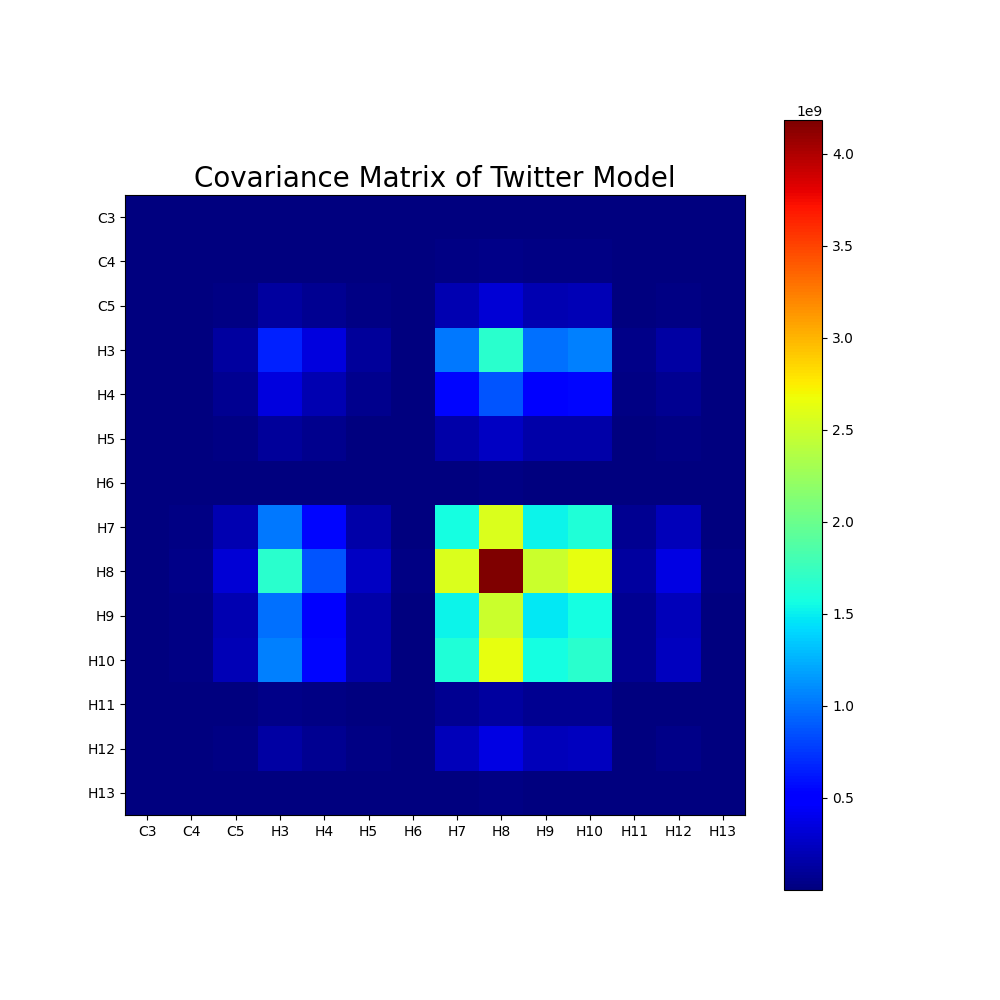
\includegraphics[width=0.6\linewidth]{../Images/CovMatTwitterModel020209.png}
        \centering
    \end{figure}
\end{frame}


\begin{frame}
    \frametitle{Thij Model $\lambda=0.2$, $p=0.8$}
    \begin{figure}
        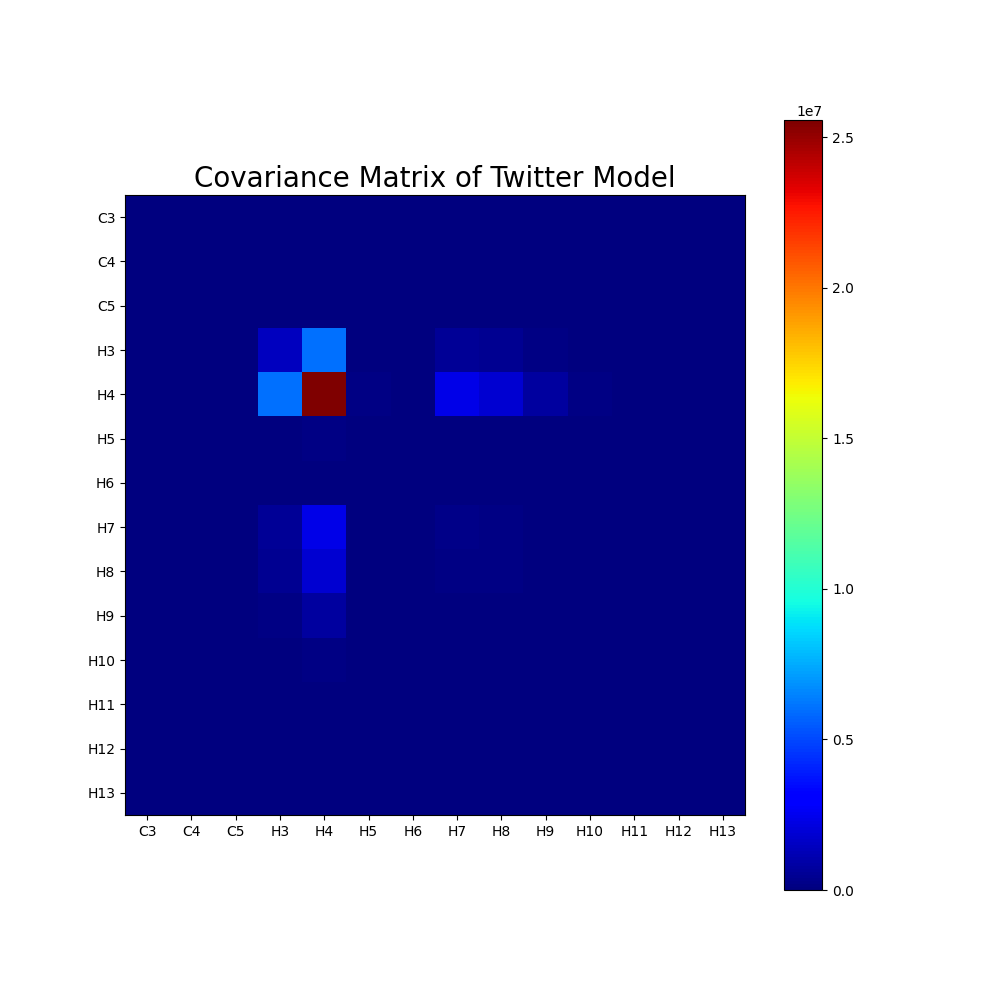
\includegraphics[width=0.6\linewidth]{../Images/CovMatTwitterModel020809.png}
        \centering
    \end{figure}
\end{frame}

\begin{frame}
    \frametitle{Thij Model $\lambda=0.8$, $p=0.2$}
    \begin{figure}
        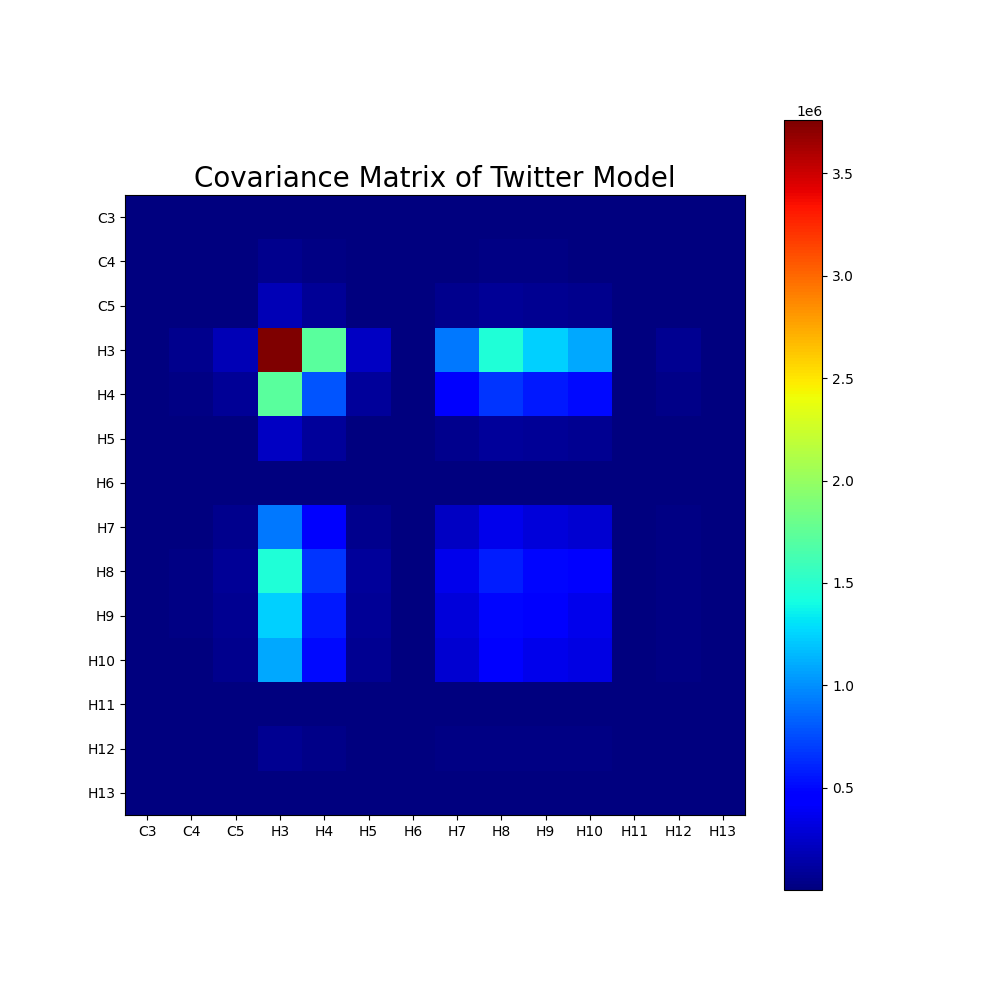
\includegraphics[width=0.6\linewidth]{../Images/CovMatTwitterModel080209.png}
        \centering
    \end{figure}
\end{frame}


\begin{frame}
    \frametitle{Thij Model $\lambda=0.8$, $p=0.8$}
    \begin{figure}
        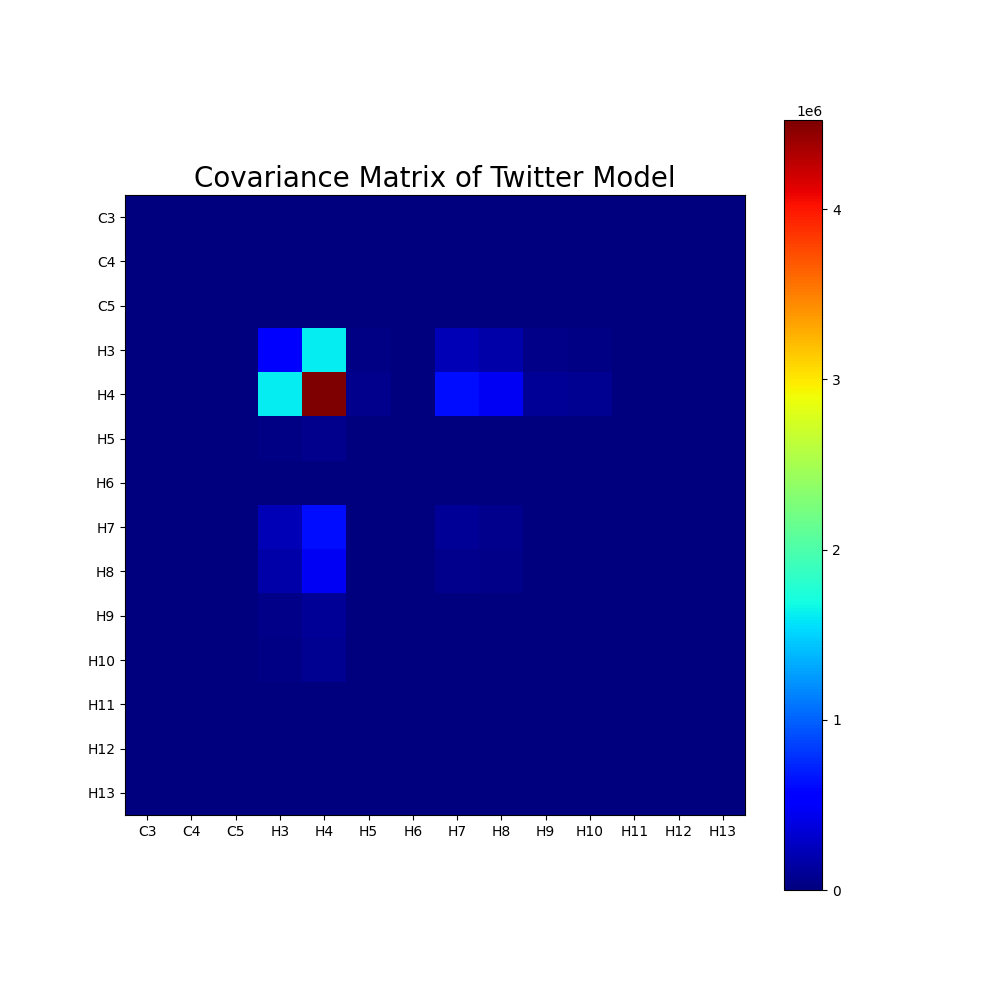
\includegraphics[width=0.6\linewidth]{../Images/CovMatTwitterModel080809.png}
        \centering
    \end{figure}
\end{frame}


%%%%%%%%%%%%%%%%%%%%%%%%%%%%%%%%%%%%%%%%%%%%%%%%%%%%%%%%%%%%%%%%%%%%%%%%%%%%%%%%%%%%%%%%%%%%%%%%%%%%%%%
%%%%%%%%%%%%%%% Koopman Operator
%%%%%%%%%%%%%%%%%%%%%%%%%%%%%%%%%%%%%%%%%%%%%%%%%%%%%%%%%%%%%%%%%%%%%%%%%%%%%%%%%%%%%%%%%%%%%%%%%%%%%%%

\section{Dynamic Mode Decomposition and The Koopman Operator}

\begin{frame}
    \frametitle{The Koopman Operator}
    The Koopman Operator underlies the theory of the Dynamical Mode Decomposition \cite{brunton2021modern}.

\vspace{3mm}

Suppose we have non-linear, continuous dynamical system.

    $$
\frac{dy}{dt} = f(y) \quad y(0) = x \in \mathbb{R}^N
$$

\noindent with $N\gg1$. $y(t)$ is the state of the dynamical system at time $t$. Sampling the dynamical
system every $\Delta t$ we get the discrete time-series

$$
y_{k+1} = F(y_k)\
$$

We seek a coordinate transformation that renders the dynamical system much easier to evaluate.

\end{frame}

\begin{frame}
\frametitle{The Koopman Operator}
\begin{definition}[The Koopman Operator]
    We define a Hilbert space of observables $ L_2(O) = L_2(\mathbb{R}^N, \mathbb{R}, \mu)$, with an associated norm 
    $\int_{\mathbb{R}^N} |g(x) |^2 d\mu(x)  < \infty$, where $\mu$ is some appropriately chosen measure. The Koopman
    operator $K : L_2(O) \rightarrow L_2(O)$ is a mapping between the Hilbert space of observables unto itself, such that
    $$
    Kg(x_k) = g(F(x_k)) = g(x_{k+1}), \quad g \in L_2(O),
    $$

    \noindent where $F:\mathcal{M}\rightarrow \mathcal{M}$, where $\mathcal{M}$ is a smooth $n$-dimensional manifold.
\end{definition}

We are able trade a non-linear, finite-dimensional dynamical system for the linear, infinite-dimensional Koopman Operator.

\end{frame}

\begin{frame}
    \frametitle{Koopman Eigenfunctions}
    A Koopman eigenfunction $\varphi(x)$ satistfies

    $$
        K\varphi(x) = \mu \varphi(x)
    $$
    We can write any observable $g(x_k)$ in terms of an eigenfunction expansion.
    $$
    g(x_k) = \sum^{\infty}_{j=1} \varphi_{j}(x_k) \xi_{j}
    $$

    Moreover, we can evolve in the space of observables like so:

    $$
    Kg(x_k) = g(x_{k+1}) =  \sum^{\infty}_{j=1} \mu_j \varphi_{j}(x_k) \xi_{j}
    $$
\end{frame}


%%%%%%%%%%%%%%%%%%%%%%%%%%%%%%%%%%%%%%%%%%%%%%%%%%%%%%%%%%%%%%%%%%%%%%%%%%%%%%%%%%%%%%%%%%%%%%%%%%%%%%%
%%%%%%%%%%%%%%% DMD
%%%%%%%%%%%%%%%%%%%%%%%%%%%%%%%%%%%%%%%%%%%%%%%%%%%%%%%%%%%%%%%%%%%%%%%%%%%%%%%%%%%%%%%%%%%%%%%%%%%%%%%


\begin{frame}
    \frametitle{Dynamic Mode Decomposition}
    Let us define a matrix of snapshots X. 

    $$
    X = [x_1, x_2, x_3,\dots, x_n]
    $$
    
    $x_i$ denotes the state space of our dynamic system at time $i \delta t$. Our dictionary of observables is defined by the function $g(x_i)$. 
    $$
    G = [g(x_1), g(x_2), \dots, g(x_n)]
    $$

    From $G$ we produce two matrices $G_{+}$ and $G_{-}$

    \begin{align*}
        G_{+} &= [g(x_2), g(x_3), \dots, g(x_n)]\\
      G_{-} &= [g(x_1), g(x_2), \dots, g(x_{n-1})] 
    \end{align*}
\end{frame}

\begin{frame}
    \frametitle{Dynamic Mode Decomposition Cont.}
    Now suppose there is a matrix $A$ which moves the system forward one step in time, that is:

    $$
    G_{+} = AG_{-}
    $$
    $$
    A = G_{+}G^{\dagger}_{-}
    $$

    We apply the r-rank Singular Value Decomposition to $G_{-}$.

    \begin{align*}
        G_{+} = {\tilde A}U_r S_r V_r \\
        {\tilde A} = G_{+}V^{T}_r S^{-1}_r U^{T}_r
    \end{align*}

    An eigendecomposition of ${\tilde A}$ produces the DMD modes $\xi_j$ and eigenvalues $\mu_j$ \cite{doi:10.1137/1.9781611974508}.
\end{frame}
\begin{frame}
    \frametitle{SVD Truncation}
     Using the parameter $\alpha$
    we truncate the SVD. We take the r-rank SVD, whose singular values $\sigma_i$ $i=0,1,2,3\dots n$ ,satisfy
    $$
    -\alpha > \log_{10} \left(\frac{\sigma_i}{\max(\sigma_i)}\right)
    $$

    Thus we only find a small set of DMD modes relative to the maximum singular value of the SVD. 
\end{frame}

\begin{frame}
    \frametitle{The DMD Modes}
    The DMD modes $\xi_j$ show spatiotemporal coherent structures that have associated temporal behaviors (growth, decay, oscillation)
    via the DMD eigenvalues $\mu_j$.

    \vspace{3mm}
    
    When plotting the DMD modes and DMD eigenvalues, we also compute the
     eigenfunction values $\varphi_j(x_k) \quad \text{for } k=0,1,2,\dots,n$. 

    \vspace{3mm}

    We compute the eigenfunction values via the linear algebra problem 
    $$\varPhi \Psi = G$$
     solving for the matrix $\varPhi$. The column vectors of $\Psi$
    are the DMD modes $\xi_j$.

\end{frame}

%%%%%%%%%%%%%%%%%%%%%%%%%%%%%%%%%%%%%%%%%%%%%%%%%%%%%%%%%%%%%%%%%%%%%%%%%%%%%%%%%%%%%%%%%%%%%%%%%%%%%%%
%%%%%%%%%%%%%%% KDMD
%%%%%%%%%%%%%%%%%%%%%%%%%%%%%%%%%%%%%%%%%%%%%%%%%%%%%%%%%%%%%%%%%%%%%%%%%%%%%%%%%%%%%%%%%%%%%%%%%%%%%%%

\begin{frame}
    \frametitle{Kernel Dynamic Mode Decomposition}
    Many optimization problems have a dual representation in terms of kernel functions \cite{williams2015kernelbased}.

    \begin{definition}[Kernel Function]
        We define the kernel function $k:\mathbb{R}^n \times \mathbb{R}^n \rightarrow \mathbb{R}$, $ k(x,{\hat x}) = \langle \phi(x), \phi({\hat x})\rangle$.
        $k$ maps a pair of vectors to an inner product of observables of the data.
    \end{definition}

    We are able to represent non-linear terms built from the state-space in the inner-product of $x, {\hat x}$. In
    this thesis, we use the polynomial kernel.

    $$
    k(x,x') = (1 + x^Tx')^p
    $$

    We take $p=2$ for each application of KDMD.
\end{frame}
\begin{frame}
    \frametitle{Kernel Dynamic Mode Decomposition}
    We form the matrices $\Phi^{+}$, $\Phi^{-}$ from our snapshot matrix: X.
    First. recall the pair of snapshot matrices $X^{+}$, $X^{-}$.
    \begin{align*}
        X^{+} = [x_1,x_2,\dots,x_n]\\
        X^{-} = [x_0,x_1,\dots,x_{n-1}]
    \end{align*}
    Then the $i$th row, $j$th column element of $\Phi^{+}$, $\Phi^{-}$ is given by:

    \begin{align*}
        \Phi^{+}_{i,j} = k(X^{+}_i,X^{-}_j)\\
        \Phi^{-}_{i,j}= k(X^{-}_i,X^{-}_j)
    \end{align*}
\end{frame}

\begin{frame}
    \frametitle{The KDMD Modes}
    We take the r-rank SVD of $\Phi^{-}=U_r S_r V_r$ using the same method of truncation.
     So now we calculate the matrix
    $$
    {\hat K} = (S^{-1}_r U^T_r)\Phi^{+}(U_r S^{-1}_r)
    $$
    Taking the eigendecomposition of $\hat K$, let $\hat \Psi$ denote the matrix
    whose column vectors are eigenvectors of ${\hat K}$.
    We can find $\varphi(x_k)$ via the $k$th column of the matrix multiplication 

    $$
        \varPhi = U_r S_r {\hat \Psi}
    $$

    The DMD modes are found in the columns of $\Psi$ given by the matrix equation:

    $$
    Y = \varPhi \Psi.
    $$
\end{frame}

\begin{frame}
    \frametitle{One-Step Reconstruction Error}
    First, we define the one-step reconstruction
    error $u$. We define the matrix ${\tilde G}$ where the $j$th column vectors of ${\tilde G}$ are the one-step
    reconstructions of the state space at time $j$ for $j=1,2,\dots, n$.
    
    $$
    {\tilde G}_{j} = \sum^{r}_{k} \mu_k \varphi_k(x_{j-1}) \xi_k
    $$
    
    $$
    u = \frac{\|G_{+} - {\tilde G} \|_F}{\|G_{+}\|_F}
    $$
\end{frame}

\begin{frame}
    \frametitle{Mode Error (Rowley Measure)}
    Provided that $\varphi_j$ and $\mu_j$ are
a true eigenpair it follows \cite{zhang2017evaluating}:

$$
\varphi_j \circ F = \mu_j \varphi_j
$$

\noindent Letting $\|\cdot\|$ denote the $L_2$ norm, we would like to calculate 

$$
\frac{\| \varphi_j \circ F - \mu \varphi_j \|}{\| \varphi_j \|}
$$

\noindent However, if we know $F$, then DMD is not a useful tool.
We must estimate $F$ using a finite number of data points. We take
two data points $x_k, x_{k+1} \in X$. We can now write 

$$
{\tilde r}_{j} = \frac{\sum_{k} |\varphi_j(x_{k+1}) - \mu_j \varphi_j(x_{k})|}{\sum_{k} |\varphi_j(x_k )|}
$$

\end{frame}

\begin{frame}
\frametitle{Data Preprocessing}
In order to improve the fit of the DMD and KDMD algorithms to the data, we distribute the interarrival times between events according
to an exponential process $g(x;\gamma)$.

$$
g(x;\gamma) = \gamma e^{ - \gamma x}
$$

\vspace{3mm}
We take $\gamma=10$. We then smooth the data with a window average. We then take the last ten thousand time-steps of each simulation to run DMD and KDMD on. 
This limits the impact of the dimensionality problem on KDMD. Finally, we also center the data about the mean.
\end{frame}

\section{Results}
%%%%%%%%%%%%%%%%%%%%%%%%%%%%%%%%%%%%%%%%%%%%%%%%%%%%%%%%%%%%%%%%%%%%%%%%%%%%%%%%%%%%%%%%%%%%%%
\begin{frame}
    \frametitle{DMD Results for BA Model with $k=1$}
    \begin{figure}
        \includegraphics[width = 0.4\linewidth]{../Images/DMDm1k300eigen-2.png}
        \centering
    \end{figure}
\end{frame}

\begin{frame}
    \frametitle{KDMD Results for BA Model with $k=1$}
    \begin{figure}
        \includegraphics[width = 0.4\linewidth]{../Images/KDMDm1k300eigen-2.png}
        \centering
    \end{figure}
\end{frame}

\begin{frame}
    \frametitle{Errors for BA Model with $k=1$}
    \begin{itemize}
        \item  Reconstruction error for DMD: $0.97$. 
        \item  Reconstruction error for KDMD: $0.036$.
    \end{itemize}
   
    \begin{figure}
        \includegraphics[width = 0.9\linewidth]{../Images/Pref_Mode_errors1.png}
        \centering
    \end{figure}
\end{frame}
%%%%%%%%%%%%%%%%%%%%%%%%%%%%%%%%%%%%%%%%%%%%%%%%%%%%%%%%%%%%%%%%%%%%%%%%%%%%%%%%%%%%%%%%%%%%%%

\begin{frame}
    \frametitle{DMD Results for BA Model with $k=2$}
    \begin{figure}
        \includegraphics[width = 0.4\linewidth]{../Images/DMDm2k300eigen-2.png}
        \centering
    \end{figure}
\end{frame}

\begin{frame}
    \frametitle{KDMD Results for BA Model with $k=2$}
    \begin{figure}
        \includegraphics[width = 0.4\linewidth]{../Images/KDMDm2k300eigen-2.png}
        \centering
    \end{figure}
\end{frame}

\begin{frame}
    \frametitle{Errors for BA Model with $k=2$}
    \begin{itemize}
        \item  Reconstruction error for DMD: $0.97$. 
        \item  Reconstruction error for KDMD: $0.0156$.
    \end{itemize}
   
    \begin{figure}
        \includegraphics[width = 0.9\linewidth]{../Images/Pref_Mode_errors2.png}
        \centering
    \end{figure}
\end{frame}
%%%%%%%%%%%%%%%%%%%%%%%%%%%%%%%%%%%%%%%%%%%%%%%%%%%%%%%%%%%%%%%%%%%%%%%%%%%%%%%%%%%%%%%%%%%%%%

\begin{frame}
    \frametitle{DMD Results for Thij Model with $\lambda=0.2$, $p=0.2$}
    \begin{figure}
        \includegraphics[width = 0.4\linewidth]{../Images/DMD_twitter_020209-2.png}
        \centering
    \end{figure}
\end{frame}

\begin{frame}
    \frametitle{KDMD Results for Thij Model with $\lambda=0.2$, $p=0.2$}
    \begin{figure}
        \includegraphics[width = 0.4\linewidth]{../Images/KDMD_twitter_020209-2.png}
        \centering
    \end{figure}
\end{frame}

\begin{frame}
    \frametitle{Errors for Thij Model with $\lambda=0.2$, $p=0.2$}
    \begin{itemize}
        \item  Reconstruction error for DMD: $0.99$. 
        \item  Reconstruction error for KDMD: $0.108$.
    \end{itemize}
   
    \begin{figure}
        \includegraphics[width = 0.9\linewidth]{../Images/Mode_errors4.png}
        \centering
    \end{figure}
\end{frame}
%%%%%%%%%%%%%%%%%%%%%%%%%%%%%%%%%%%%%%%%%%%%%%%%%%%%%%%%%%%%%%%%%%%%%%%%%%%%%%%%%%%%%%%%%%%%%%
\begin{frame}
    \frametitle{DMD Results for Thij Model with $\lambda=0.2$, $p=0.8$}
    \begin{figure}
        \includegraphics[width = 0.4\linewidth]{../Images/DMD_twitter_020809-2.png}
        \centering
    \end{figure}
\end{frame}

\begin{frame}
    \frametitle{KDMD Results for Thij Model with $\lambda=0.2$, $p=0.8$}
    \begin{figure}
        \includegraphics[width = 0.4\linewidth]{../Images/KDMD_twitter_020809-2.png}
        \centering
    \end{figure}
\end{frame}

\begin{frame}
    \frametitle{Errors for Thij Model with $\lambda=0.2$, $p=0.8$}
    \begin{itemize}
        \item  Reconstruction error for DMD: $0.96$. 
        \item  Reconstruction error for KDMD: $0.053$.
    \end{itemize}
   
    \begin{figure}
        \includegraphics[width = 0.9\linewidth]{../Images/Mode_errors2.png}
        \centering
    \end{figure}
\end{frame}
%%%%%%%%%%%%%%%%%%%%%%%%%%%%%%%%%%%%%%%%%%%%%%%%%%%%%%%%%%%%%%%%%%%%%%%%%%%%%%%%%%%%%%%%%%%%%%
\begin{frame}
    \frametitle{DMD Results for Thij Model with $\lambda=0.8$, $p=0.2$}
    \begin{figure}
        \includegraphics[width = 0.4\linewidth]{../Images/DMD_twitter_080209-2.png}
        \centering
    \end{figure}
\end{frame}

\begin{frame}
    \frametitle{KDMD Results for Thij Model with $\lambda=0.8$, $p=0.2$}
    \begin{figure}
        \includegraphics[width = 0.4\linewidth]{../Images/KDMD_twitter_080209-2.png}
        \centering
    \end{figure}
\end{frame}

\begin{frame}
    \frametitle{Errors for Thij Model with $\lambda=0.8$, $p=0.2$}
    \begin{itemize}
        \item  Reconstruction error for DMD: $0.99$. 
        \item  Reconstruction error for KDMD: $0.0076$.
    \end{itemize}
   
    \begin{figure}
        \includegraphics[width = 0.9\linewidth]{../Images/Mode_errors3.png}
        \centering
    \end{figure}
\end{frame}
%%%%%%%%%%%%%%%%%%%%%%%%%%%%%%%%%%%%%%%%%%%%%%%%%%%%%%%%%%%%%%%%%%%%%%%%%%%%%%%%%%%%%%%%%%%%%%

\begin{frame}
    \frametitle{DMD Results for Thij Model with $\lambda=0.8$, $p=0.8$}
    \begin{figure}
        \includegraphics[width = 0.4\linewidth]{../Images/DMD_twitter_080809-2.png}
        \centering
    \end{figure}
\end{frame}

\begin{frame}
    \frametitle{KDMD Results for Thij Model with $\lambda=0.8$, $p=0.8$}
    \begin{figure}
        \includegraphics[width = 0.4\linewidth]{../Images/KDMD_twitter_080809-2.png}
        \centering
    \end{figure}
\end{frame}

\begin{frame}
    \frametitle{Errors for Thij Model with $\lambda=0.8$, $p=0.8$}
    \begin{itemize}
        \item  Reconstruction error for DMD: $0.943$. 
        \item  Reconstruction error for KDMD: $0.0524$.
    \end{itemize}
   
    \begin{figure}
        \includegraphics[width = 0.9\linewidth]{../Images/Mode_errors4.png}
        \centering
    \end{figure}
\end{frame}
%%%%%%%%%%%%%%%%%%%%%%%%%%%%%%%%%%%%%%%%%%%%%%%%%%%%%%%%%%%%%%%%%%%%%%%%%%%%%%%%%%%%%%%%%%%%%%

\section{Conclusion}

\begin{frame}
    \frametitle{Possible Applications}
    \begin{itemize}
        \item DMD modes could be used to classify different networks by their local temporal dynamics.
        \item DMD modes could be used to classify types of Twitter behavior (bots vs. people) \cite{ferrara2020covid} \cite{bovet2019influence} \cite{Grant}.
    \end{itemize}
    \end{frame}

\begin{frame}
\frametitle{Future Study}
\begin{itemize}
    \item The error of the DMD could be improved through EDMD, by judiciously selecting $g$. 
    \item There are many kernel functions for KDMD. Different basis functions may produce better results. 
    \item We also may wish to examine the inner products between modes to study motif interaction.
\end{itemize}
\end{frame}

\begin{frame}[allowframebreaks]
    \frametitle{References}
    \bibliographystyle{siam}
    \bibliography{../thbib.bib}
\end{frame}


\appendix %do not count the following slides for the total number

\begin{frame}
    \frametitle{Appendix: Counting Motifs}
extra slide 1
\end{frame}

\begin{frame}
    \frametitle{Appendix: Counting Motifs}
extra slide 2
\end{frame}

\begin{frame}
    \frametitle{Appendix: $k=1$ Results}
    \begin{figure}
        \includegraphics[width=0.6\linewidth]{../Images/graph_stats_pref_attach_8_1_300.png}
    \centering
    \end{figure}
\end{frame}

\begin{frame}
    \frametitle{Appendix: $k=1$ Network}
    \begin{figure}
        \includegraphics[width=0.7\linewidth]{../Images/final_pref1_centrality.png}
    \centering
    \end{figure}
\end{frame}

\begin{frame}
    \frametitle{Appendix: $k=2$ Statistics}
    \begin{figure}
        \includegraphics[width=0.6\linewidth]{../Images/graph_stats_pref_attach_10_2_300.png}
    \centering
    \end{figure}
\end{frame}

\begin{frame}
    \frametitle{Appendix: $k=2$ Network}
    \begin{figure}
        \includegraphics[width=0.7\linewidth]{../Images/final_pref2_centrality.png}
    \centering
    \end{figure}
\end{frame}

\end{document}